% ============================================================================
% Detection Is Not Attribution -- ICASSP 2027 satellite workshop (C4AI4C) submission
% Build: pdflatex main; bibtex main; pdflatex main; pdflatex main   (or Overleaf, pdfLaTeX)
% Every number is taken from the frozen artifacts in data/ and the verified Claude asset package
% (PROVENANCE.json). Figures are regenerated from data/*.csv by scripts/make_figures.py.
% AUTHOR CHECK before submission: e-mails, ORCID IDs, funding, AI-use wording, NDSS prior-submission status.
% ============================================================================
\documentclass{article}
\usepackage{spconf,amsmath,amssymb,graphicx,booktabs,microtype}
\usepackage[table]{xcolor}
\usepackage{pifont}
\usepackage{algorithm,algpseudocode}
\usepackage[hidelinks]{hyperref}
% Shared colour palette (figures and shaded tables)
\definecolor{cliC}{HTML}{EEF2F8}\definecolor{attC}{HTML}{FBE3E0}\definecolor{attD}{HTML}{C0392B}
\definecolor{magC}{HTML}{E4EDFA}\definecolor{temC}{HTML}{E3F2E3}\definecolor{fusC}{HTML}{FDF1D6}
\definecolor{srvC}{HTML}{F8F8F8}\definecolor{verC}{HTML}{EFE8F7}\definecolor{audC}{HTML}{FBF5E6}
% outcome cells
\definecolor{okC}{HTML}{CFE8C6}\definecolor{okfaC}{HTML}{E9F0BE}\definecolor{wC}{HTML}{FCDDAE}
\definecolor{mC}{HTML}{E2E2E2}\definecolor{faC}{HTML}{F5C6C0}
% outcome-cell macros (used by tables/*.tex)
\newcommand{\cOK}[1]{\cellcolor{okC}\ding{51}\,#1}
\newcommand{\cOKF}[2]{\cellcolor{okfaC}\ding{51}\,#1\,+F$_{#2}$}
\newcommand{\cW}[2]{\cellcolor{wC}W$_{#1}$\,#2}
\newcommand{\cM}{\cellcolor{mC}M}
\newcommand{\cMF}[1]{\cellcolor{faC}M+F$_{#1}$}
\newcommand{\cF}[1]{\cellcolor{faC}F$_{#1}$}
\newcommand{\cN}{--}
\newcommand{\grp}[2]{\multicolumn{#1}{@{}l}{\rule{0pt}{2.4ex}\textit{#2}}\\[-0.2ex]}
\newcommand{\wst}{$^\ast$}

% V9: tighter spacing between floats (figures/tables/algorithm) and the surrounding text
\setlength{\textfloatsep}{7pt plus 2pt minus 2pt}
\setlength{\floatsep}{6pt plus 2pt minus 2pt}
\setlength{\dbltextfloatsep}{7pt plus 2pt minus 2pt}
\setlength{\dblfloatsep}{6pt plus 2pt minus 2pt}
\setlength{\intextsep}{6pt plus 2pt minus 2pt}
\setlength{\abovecaptionskip}{3pt}
\setlength{\belowcaptionskip}{0pt}

\title{Detection Is Not Attribution: A Matched Reliability Audit of\\ Federated-Learning Forensics Under Poisoning and Benign Drift}
\twoauthors
  {Al Amin}
  {Huston--Tillotson University\\ Austin, TX, USA\\ \texttt{aamin@htu.edu}}
  {Kamrul Hasan, Liang Hong}
  {Tennessee State University\\ Nashville, TN, USA\\ % AUTHOR: add coauthor e-mails here
   }

\begin{document}
\ninept
\maketitle

\begin{abstract}
A server-side forensic monitor for federated learning (FL) must do more than flag an anomaly: it must name the right client, date the intervention, and leave honest clients alone. We audit a frozen monitor, FedTrace~v3, together with three sequential norm detectors, under matched clean, BadNets, relabel-only and honest class-drift arms that share bit-identical histories before the intervention. On a five-client CIFAR-100 setup with four seeds (two preregistered), FedTrace~v3 raises no clean alarm but misses the BadNets attacker on both confirmation seeds, including a run with 63.3\% attack success. Norm z-score persistence and CUSUM name the attacker in all four BadNets runs yet accuse honest clients in every drift run and in one clean run. A peer-median displacement explains a misattribution on one development seed only. We report these as seed-level failures, not population error rates.
\end{abstract}

\begin{keywords}
federated learning, forensic attribution, data poisoning, benign drift, sequential change detection
\end{keywords}

% ----------------------------------------------------------------------------
\section{Introduction}
\label{sec:intro}

Federated learning (FL) trains a shared model from client updates without collecting raw data~\cite{mcmahan2017fedavg}, and heterogeneous client data already make those updates noisy~\cite{li2020fedprox,karimireddy2020scaffold}. A poisoned client can implant a backdoor~\cite{gu2019badnets,bagdasaryan2020backdoor} or bias training over many rounds~\cite{xie2025poisonedfl}. When a server-side monitor raises an alarm, the operator needs answers to five different questions: was the intervention effective, was its source detected, was the \emph{right} client named first, when did it begin, and was any honest client accused? A single detection score merges these questions. In a five-client cross-silo federation, wrongly excluding one client removes 20\% of the participants, so the last question matters as much as the first.

We audit FedTrace~v3, a monitor we developed earlier for model-update perturbations, without changing its code or thresholds (Fig.~\ref{fig:overview}). Our contributions are:
\begin{itemize}\setlength{\itemsep}{0pt}\setlength{\parsep}{0pt}\setlength{\topsep}{2pt}
\item a matched audit in which clean, BadNets, relabel-only and honest-drift arms share bit-identical pre-intervention histories, supporting controlled within-seed comparisons;
\item seed-level reporting of all five outcomes for the monitor, three norm baselines and five ablations, with two preregistered confirmation seeds;
\item a diagnosis of two failure modes, threshold transfer and a conditional peer-median displacement.
\end{itemize}
Separating the forensic outcomes is not itself new~\cite{zhang2022fldetector,zhang2024fltracer}; what we add is a matched benign-drift control and a record that keeps missed attackers, unsuccessful attacks and false accusations. Section~\ref{sec:related} reviews related work, Section~\ref{sec:monitor} defines the audited monitor and baselines, Section~\ref{sec:protocol} the matched protocol, Section~\ref{sec:results} reports the results, Section~\ref{sec:contamination} analyses the peer-median displacement, Section~\ref{sec:archived} summarizes archived model-update perturbations, and Section~\ref{sec:conclusion} concludes.

\begin{figure*}[t]
\centering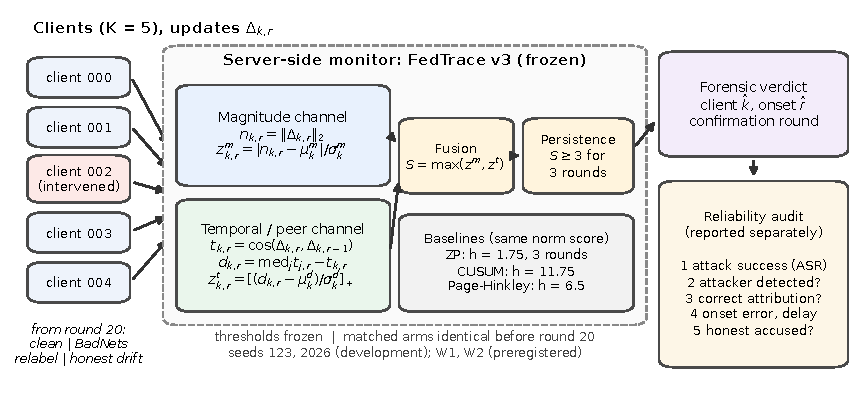
\includegraphics[width=.96\textwidth]{figures/fig_overview.pdf}
\caption{\textbf{Frozen monitor and reliability audit.} Identity-labelled updates enter the magnitude and temporal channels, maximum-score fusion, and three-round persistence. Matched clean, BadNets, relabel-only, and honest-drift arms are assessed separately for attack success, detection, first attribution, onset error/delay, and honest-client accusations.}
\label{fig:overview}
\end{figure*}

% ----------------------------------------------------------------------------
\section{Related Work}
\label{sec:related}

\textbf{Robust aggregation and detection.} Krum bounds the influence of Byzantine updates but does not attribute them~\cite{blanchard2017krum}; FoolsGold and FLTrust reweight clients by similarity or trust~\cite{fung2020foolsgold,cao2021fltrust}. DeepSight inspects update features~\cite{rieger2022deepsight}, CrowdGuard uses client-side validation~\cite{rieger2024crowdguard}, BackdoorIndicator probes server-injected indicator tasks~\cite{li2024backdoorindicator}, and FedREDefense targets crafted \emph{model} poisoning through reconstruction error~\cite{xie2024fedredefense}.

\textbf{Forensics and provenance.} FLDetector flags clients whose updates are inconsistent with their history~\cite{zhang2022fldetector}. FLTracer traces poisoning provenance and timing and notes difficulty with abrupt benign change~\cite{zhang2024fltracer}. FLForensics traces clients backwards from a misclassified target~\cite{jia2025flforensics}, and FedGT identifies malicious clients under secure aggregation by group testing~\cite{xhemrishi2025fedgt}. Our baselines are classical sequential change detectors: CUSUM~\cite{page1954cusum} and Page--Hinkley~\cite{hinkley1971change}. We did not run any published forensic system, so we make no numerical comparison with them.

% ----------------------------------------------------------------------------
\section{Audited Monitor and Baselines}
\label{sec:monitor}

At round $r$ the server observes the identity-labelled update $\Delta_{k,r}\in\mathbb{R}^d$ of client $k$, but no client data. Let $n_{k,r}=\|\Delta_{k,r}\|_2$, let $t_{k,r}$ be the cosine between $\Delta_{k,r}$ and $\Delta_{k,r-1}$, let $c_r=\operatorname{med}_j t_{j,r}$ be the \emph{inclusive} peer median (all $K$ clients, including $k$), and let $d_{k,r}=c_r-t_{k,r}$. The frozen score is
\begin{align}
z^m_{k,r}&=\frac{|n_{k,r}-\mu^m_k|}{\sigma^m_k},\qquad
z^t_{k,r}=\Big[\frac{d_{k,r}-\mu^d_k}{\sigma^d_k}\Big]_+,\nonumber\\
S_{k,r}&=\max\{z^m_{k,r},\,z^t_{k,r}\},
\label{eq:monitor}
\end{align}
with per-client means and sample standard deviations from rounds 0--19 (norm) and 1--19 (residual), $T_{\rm ref}=20$. Because $z^m$ is absolute, both unusually small and unusually large updates count. Algorithm~\ref{alg:fedtrace} gives the confirmation rule: a client is confirmed after $P=3$ consecutive rounds with $S_{k,r}\ge\tau=3$; the earliest confirmed client is the attributed source (ties go to the larger mean streak score), the first round of its streak is the onset estimate $\hat r$, and the last is the confirmation round.

% Algorithm box for the frozen monitor. Verified line by line against src/analysis/fedtrace_detector.py
% (compute_all_scores_v3, apply_persistence_rule_v3; frozen at commit 7f6ca8b). Requires: \usepackage{algorithm,algpseudocode}
\begin{algorithm}[t]
\caption{FedTrace v3 forensic monitor (frozen; evaluated, not proposed)}
\label{alg:fedtrace}
\footnotesize
\begin{algorithmic}[1]
\Require client updates $\Delta_{k,r}$ for $k=1,\dots,K$; $T_{\mathrm{ref}}=20$; $\tau=3$; $P=3$
\Statex \textbf{Calibration} (once, at $r=T_{\mathrm{ref}}$)
\For{each client $k$}
  \State $\mu^m_k,\sigma^m_k \gets$ mean, s.d.\ of $n_{k,r}=\Vert\Delta_{k,r}\Vert_2$, $0\le r<T_{\mathrm{ref}}$
  \State $\mu^d_k,\sigma^d_k \gets$ mean, s.d.\ of $d_{k,r}=\mathrm{med}_j\,t_{j,r}-t_{k,r}$, $1\le r<T_{\mathrm{ref}}$
\EndFor
\Statex \textbf{Monitoring} (each round $r\ge T_{\mathrm{ref}}$)
\For{each client $k$}
  \State $t_{k,r}\gets\cos(\Delta_{k,r},\Delta_{k,r-1})$;\; $c_r\gets\mathrm{med}_{j}\,t_{j,r}$ \Comment{inclusive median}
  \State $z^m_{k,r}\gets|n_{k,r}-\mu^m_k|/\sigma^m_k$;\; $z^t_{k,r}\gets\max\{0,(c_r-t_{k,r}-\mu^d_k)/\sigma^d_k\}$
  \State $S_{k,r}\gets\max(z^m_{k,r},z^t_{k,r})$
  \If{$S_{k,r'}\ge\tau$ for $P$ consecutive rounds $r'$ ending at $r$ and $k$ not yet confirmed}
    \State confirm $k$ at round $r$; onset estimate $\hat r_k\gets r-P+1$
  \EndIf
\EndFor
\State \Return attributed client $\hat k$ = earliest confirmed client (ties: larger mean streak score); $\hat r_{\hat k}$; all confirmations
\end{algorithmic}
\end{algorithm}


\textbf{Baselines.} All three baselines act on the per-client norm. Norm z-score persistence (ZP; $h=1.75$, $P=3$) computes a statistic that is numerically identical to $z^m$ on every evaluated trace (maximum difference 0), so ZP and the v3 magnitude-only ablation differ in their frozen threshold. Norm CUSUM uses $h=11.75$, $\kappa=0.5$~\cite{page1954cusum} and Page--Hinkley uses $h=6.5$, $\delta=0.5$~\cite{hinkley1971change}. Each threshold is the smallest grid value with no alarm on the two \emph{development} clean runs; this favours sensitivity and is not a false-alarm guarantee.

% ----------------------------------------------------------------------------
\section{Matched Protocol}
\label{sec:protocol}

\textbf{Setting.} FedAvg for 50 rounds on CIFAR-100 with a CIFAR-style ResNet-18~\cite{he2016resnet}; $K=5$ fully participating clients, Dirichlet $\alpha=0.1$, one local epoch, SGD with learning rate 0.01, batch 32, and a 45k/5k train/validation split. Client 002 is intervened on from round $r^\star=20$. Within a seed, all arms share bit-identical histories before the intervention (21 global states and 100 client submissions). Seeds 123 and 2026 were used for development; W1 (1178015705) and W2 (1463065807) were drawn by a fixed SHA-256 rule and preregistered after all thresholds were frozen. In W1, client 002 holds 347 target-class samples, unlike the development seeds.

\textbf{Arms.} \emph{BadNets} stamps a $3\times3$ trigger and target label 0 on 50\% of client 002's non-target-class samples; attack success rate (ASR) is measured on 9,900 triggered non-target test images, with a preregistered effectiveness criterion of ASR $\ge50\%$. \emph{Relabel-only} (development seeds) relabels the same sample indices without a trigger. \emph{Honest drift} keeps the classes covering at least 50\% of client 002's data and replaces the remaining examples with correctly labelled samples of the kept classes from the same client, leaving dataset length and optimizer steps unchanged. It is a constructed stress test, not an estimate of how often benign drift occurs.

\textbf{Outcomes.} For attacked runs we record whether the attacker is ever confirmed, the first attributed client, onset error $e=|\hat r-r^\star|$, delay $d=r_{\rm confirm}-r^\star$, and any honest confirmation. In clean and drift runs there is no attacker, so every confirmation is a false accusation. Missing onset estimates stay missing.

% ----------------------------------------------------------------------------
\section{Results}
\label{sec:results}

% Table 1. Seed-level outcomes (numbers from data/fig_reliability_matrix_data.csv and the frozen v3 asset tab_main_outcomes.tex).
\begin{table}[t]
\centering\scriptsize
\setlength{\tabcolsep}{2.6pt}\renewcommand{\arraystretch}{1.06}
\caption{\textbf{Seed-level outcomes of the frozen monitor and the norm baselines} (no pooling). \ding{51}\,$e/d$: attacker confirmed first, onset error $e$ and confirmation delay $d$ (rounds); W$_i$\,$e/d$: honest client(s) $i$ confirmed first, attacker later; M: attacker never confirmed; F$_i$: honest client(s) $i$ confirmed (a false accusation; in drift arms client 2 is the honestly drifting client); --: no client confirmed. A \ding{51} does not exclude a later honest confirmation (+F$_i$). Acc.: change in top-1 vs.\ the matched clean run (pp), or final top-1 (\%) for clean runs; single runs, no variance estimate. $^\ast$preregistered confirmation seeds.}
\label{tab:main}
\vspace{3pt}
\begin{tabular}{@{}lrrcccc@{}}
\toprule
Seed & ASR & Acc. & FedTrace v3 & ZP & CUSUM & Page--Hinkley \\
\midrule
\grp{7}{BadNets (attacker: client 2)}
123   & 43.5 & $-1.94$ & \cOK{8/10}   & \cOK{1/3}      & \cOK{0/6}      & \cMF{0} \\
2026  & 64.7 & $-0.94$ & \cW{1,4}{2/4} & \cOK{0/2}     & \cOK{0/5}      & \cMF{1} \\
W1\wst& 63.3 & $-0.96$ & \cM          & \cOKF{1/3}{4}  & \cOKF{0/6}{4}  & \cMF{4} \\
W2\wst& 44.2 & $-0.86$ & \cM          & \cOK{1/3}      & \cOK{0/6}      & \cM \\
\grp{7}{Relabel-only, no trigger (development seeds only)}
123   & 0.7  & $-1.26$ & \cM          & \cOK{1/3}      & \cOK{0/7}      & \cM \\
2026  & 0.4  & $-1.60$ & \cMF{1,4}    & \cOK{1/3}      & \cOK{0/6}      & \cMF{1} \\
\grp{7}{Honest drift (no attacker exists)}
123   &      & $-1.75$ & \cN          & \cF{2}         & \cF{2}         & \cN \\
2026  &      & $-1.79$ & \cF{1,4}     & \cF{1}         & \cF{2}         & \cF{1} \\
W1\wst&      & $-2.29$ & \cF{2}       & \cF{2,4}       & \cF{2,4}       & \cF{4} \\
W2\wst&      & $-1.47$ & \cN          & \cF{2}         & \cF{2}         & \cN \\
\grp{7}{Clean (no intervention)}
123   &      & 56.88   & \cN & \cN    & \cN    & \cN \\
2026  &      & 57.94   & \cN & \cN    & \cN    & \cN \\
W1\wst&      & 58.04   & \cN & \cF{4} & \cF{4} & \cF{4} \\
W2\wst&      & 60.22   & \cN & \cN    & \cN    & \cN \\
\bottomrule
\end{tabular}
\end{table}


Table~\ref{tab:main} lists every outcome seed by seed and distinguishes attack success (ASR), correct \emph{first} attribution, and honest accusations. In clean and drift arms every alarm is false; accuracy changes are paired single-run differences, not variance estimates. Only 2026 and W1 meet the 50\% BadNets effectiveness criterion.

\textbf{Effective attacks can be missed.} FedTrace~v3 never confirms the attacker on W1 or W2, although W1 reaches 63.3\% ASR. On 2026 it confirms honest clients 001 and 004 one round before the attacker, so the attacker is detected but not attributed. Fig.~\ref{fig:calib}a and Table~\ref{tab:calib} show why. The attacker's norm score peaks at 3.26, 3.57, 3.04 and 2.94 on the four seeds; on W1 it reaches $\tau=3$ in only two rounds and on W2 in none, so neither meets three-round persistence. Over rounds 20--49 the score exceeds ZP's $h=1.75$ in 29--30 rounds per seed, and ZP attributes all four attackers with $e\le1$. Calibrating on rounds 0--19 includes the two high-norm opening rounds, which inflates the attacker's $\sigma^m$ by 1.9--7.1$\times$ (Table~\ref{tab:calib}) and lowers its standardized score. This pattern is consistent with reduced score sensitivity, but the runs do not establish calibration inflation as a cause; the full v3 decision also includes the temporal channel. It also does not show that ZP is generally better.

\begin{figure}[t]
\centering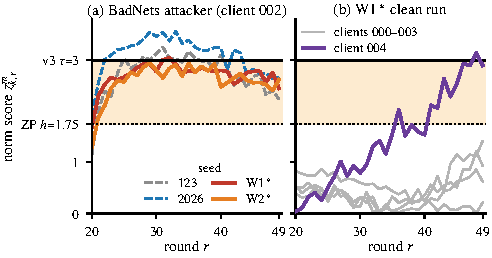
\includegraphics[width=\columnwidth]{figures/fig_calibration.pdf}
\caption{\textbf{One statistic, two thresholds.} (a) BadNets attacker (client 002): on W1$^\ast$ and W2$^\ast$ most attacker scores lie between ZP's $h=1.75$ and v3's $\tau=3$, so ZP confirms the attacker while v3 fails its three-round confirmation rule. (b) W1$^\ast$ clean run: honest client 004 drifts upward late in training and crosses $h=1.75$, coinciding with the ZP, CUSUM and Page--Hinkley clean alarms; it exceeds $\tau$ in a single round, so v3 stays silent.}
\label{fig:calib}
\end{figure}

% Table 2. Attacker norm-score statistics, BadNets arms (data/tab_calibration_data.csv).
\begin{table}[t]
\centering\scriptsize
\setlength{\tabcolsep}{4pt}
\caption{\textbf{BadNets attacker under the shared norm score} $z^m$ (rounds 20--49). v3 and ZP see the identical statistic; only the threshold differs. Inflation: attacker $\sigma^m$ over rounds 0--19 divided by $\sigma^m$ over rounds 2--19.}
\label{tab:calib}
\vspace{3pt}
\begin{tabular}{@{}lcccc@{}}
\toprule
 & 123 & 2026 & W1\wst & W2\wst \\
\midrule
Peak $z^m$                              & 3.26 & 3.57 & 3.04 & 2.94 \\
Rounds with $z^m\ge 3$ (v3 $\tau$)       & 10   & 21   & 2    & 0 \\
Rounds with $z^m>1.75$ (ZP $h$)          & 29   & 30   & 29   & 29 \\
Calibration $\sigma^m$ inflation ($\times$) & 6.28 & 7.05 & 1.92 & 6.95 \\
\bottomrule
\end{tabular}
\end{table}


\textbf{Correct attribution can coexist with false accusation.} The lower threshold has a price. ZP and CUSUM confirm honest client 004 in W1 BadNets after correctly naming the attacker, and in all four honest-drift runs they confirm a client although no attacker exists, most often the drifting client itself. In the W1 clean run ZP, CUSUM and Page--Hinkley all accuse honest client 004 (Fig.~\ref{fig:calib}b), so thresholds that were alarm-free on the development clean runs did not transfer. Page--Hinkley never confirms a BadNets attacker and accuses an honest client in three of the four BadNets runs. FedTrace~v3 raises no clean alarm on any seed but accuses honest clients in the 2026 and W1 drift runs. These runs are not independent trials: clean norm scores have lag-one autocorrelation 0.82--0.91 and cross-client correlation of about 0.94--0.95, giving an AR(1) effective sample size of 1.5--2.9 out of 30 clean monitoring rounds per client, and ZP's threshold lies only 0.031 above the largest development clean score.

\textbf{No ablation is uniformly safe.} Table~\ref{tab:ablation} keeps $\tau$ and $P$ and changes one component at a time. The magnitude-only variant attributes both development attackers correctly but still misses W1 and W2; the temporal-only variant misses every BadNets attacker and accuses honest clients on 2026. Leave-one-out and trimmed-mean references repair the 2026 attribution but name the wrong client first on 123 and add honest alarms on W1. The client-historical reference accuses honest clients in every clean run. No single reference choice avoids both misses and false accusations in these runs.

% Table 3. Frozen ablations of v3 (same thresholds). Numbers from data/fig_reliability_matrix_data.csv.
\begin{table}[t]
\centering\scriptsize
\setlength{\tabcolsep}{2.4pt}\renewcommand{\arraystretch}{1.06}
\caption{\textbf{Frozen ablations of FedTrace v3} (same $\tau$, $P$; full v3 in Table~\ref{tab:main}). Notation as in Table~\ref{tab:main}. Mag./Temp.: magnitude or temporal channel only; LOO, Trim., Hist.: leave-one-out, trimmed-mean and client-historical references instead of the inclusive median.}
\label{tab:ablation}
\vspace{3pt}
\begin{tabular}{@{}lccccc@{}}
\toprule
Seed & Mag.\ only & Temp.\ only & LOO ref. & Trim.\ ref. & Hist.\ ref. \\
\midrule
\grp{6}{BadNets}
123    & \cOK{8/10} & \cM        & \cW{1}{8/10} & \cW{1}{8/10} & \cOKF{8/10}{1,3,4} \\
2026   & \cOK{2/4}  & \cMF{1,4}  & \cOK{2/4}    & \cOK{2/4}    & \cOKF{2/4}{4} \\
W1\wst & \cM        & \cM        & \cMF{3}      & \cMF{3}      & \cMF{0,1,3,4} \\
W2\wst & \cM        & \cM        & \cM          & \cM          & \cMF{1,3} \\
\grp{6}{Relabel-only}
123    & \cM        & \cM        & \cMF{1}      & \cMF{1}      & \cMF{1,3,4} \\
2026   & \cM        & \cMF{1,4}  & \cM          & \cM          & \cMF{4} \\
\grp{6}{Honest drift}
123    & \cN        & \cN        & \cF{1}       & \cF{1}       & \cF{1,3,4} \\
2026   & \cN        & \cF{1,4}   & \cN          & \cN          & \cF{4} \\
W1\wst & \cF{2}     & \cN        & \cF{2,3,4}   & \cF{2,4}     & \cF{0,1,2,3,4} \\
W2\wst & \cN        & \cN        & \cN          & \cN          & \cF{1,3} \\
\grp{6}{Clean}
123    & \cN & \cN & \cN & \cN & \cF{1,3,4} \\
2026   & \cN & \cN & \cN & \cN & \cF{2,4} \\
W1\wst & \cN & \cN & \cN & \cN & \cF{0,2,3,4} \\
W2\wst & \cN & \cN & \cN & \cN & \cF{1,3} \\
\bottomrule
\end{tabular}
\end{table}


% ----------------------------------------------------------------------------
\begin{figure*}[t]
\centering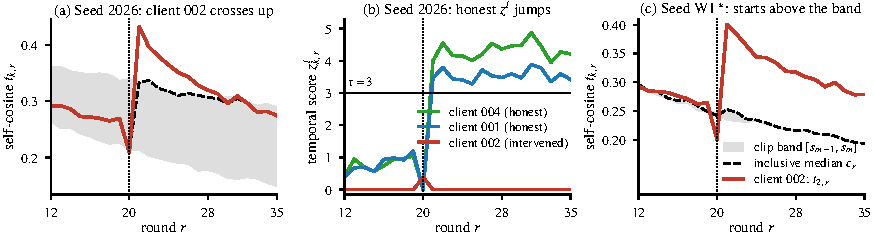
\includegraphics[width=\textwidth]{figures/fig_contamination.pdf}
\caption{\textbf{Conditional peer-median displacement.} (a) Seed 2026: client 002 is the median-ranked client before onset; at round 21 its self-cosine jumps to 0.43 and drags the inclusive median $c_r$ up within the clip band of Eq.~(\ref{eq:clip}). (b) The honest clients' temporal scores jump above $\tau=3$ while the intervened client's stays at 0. (c) Seed W1$^\ast$: client 002 already sits above the band, so the precondition fails. One-seed retrospective explanation, not a general causal claim.}
\label{fig:contam}
\end{figure*}

\section{Conditional Peer-Median Displacement}
\label{sec:contamination}

Why does v3 accuse honest clients on 2026? Let $j$ be the intervened client with self-cosine $x=t_{j,r}$, hold the honest self-cosines fixed, and sort the other $K-1$ values as $s_1\le\cdots\le s_{K-1}$ with $K=2m-1$. The inclusive median then obeys the elementary clip identity
\begin{equation}
c(x)=\min\{\max\{x,s_{m-1}\},s_m\},\qquad
\frac{\Delta d_{k,r}}{\sigma^d_k}=\frac{\Delta c_r}{\sigma^d_k}\quad(k\neq j).
\label{eq:clip}
\end{equation}
An upward move of $x$ can thus raise every honest residual by the same amount, and the shift reaches $z^t$ while the one-sided score is positive. A reference shift alone is insufficient for a verdict: the one-sided temporal score must remain above threshold for three consecutive rounds.



On 2026, client 002 held median rank 3/5 before onset. At round 21 its self-cosine rose to 0.43 and the reference moved from the matched-clean 0.257 to 0.333 (Fig.~\ref{fig:contam}a). The honest standardized residuals shifted by $+1.3$ to $+2.4$ SD on average over rounds 20--29, with temporal scores of 3.4--4.6 in rounds 21--23 (Fig.~\ref{fig:contam}b). Removing this shift retrospectively takes at least one round out of each of six related honest confirming streaks (three intervention arms $\times$ two honest clients), compared with three of six explained by the observed reference movement alone. On the other seeds client 002 held rank 4/5 before onset, so this upward-crossing precondition was absent (Fig.~\ref{fig:contam}c). This is therefore not evidence that the same mechanism caused the W1/W2 misses, nor a validated real-time correction: a deployable proxy for this displacement had a mean error of 0.07$z$ in development but 0.6--2.7$z$ on the confirmation seeds, so it is not reliable enough to deploy.

% ----------------------------------------------------------------------------
\section{Archived Model-Update Perturbations}
\label{sec:archived}

% Table 4. Archived model-update perturbations (frozen v3; tab_archived.tex and tab_sensitivity.tex assets).
\begin{table}[t]
\centering\scriptsize
\setlength{\tabcolsep}{3pt}
\caption{\textbf{Archived model-update perturbations} (not local-data poisoning; FedAvg, frozen v3). Top: onset error / delay (rounds); attribution correct in every perturbation row; F: honest client confirmed. Bottom: archived $(\tau,P)$ sweep, reported as correct attributions out of 4; runs with an honest alarm.}
\label{tab:archived}
\vspace{3pt}
\begin{tabular}{@{}lcc@{}}
\toprule
Setting & Seeds & $e/d$ \\
\midrule
Gaussian noise, $\rho=1$, $K=5$                 & 123, 2026 & 0/2, 0/2 \\
Norm-preserving directional, $c=0$, $K=5$       & 123, 2026 & 0/2, 0/2 \\
Directional; attacker 004 / onset round 30      & 123       & 0/2, 0/2 \\
Gaussian / directional, $K=10$                  & 123       & 0/2, 0/2 \\
Reduced severity: Gaussian $\rho=0.5$           & 123       & \cellcolor{wC}21/23 \\
Reduced severity: directional $c=0.5$           & 123       & 0/2 \\
Intermittent Gaussian / directional             & 123       & 0/2, 0/2 \\
Ablation: magnitude only, directional           & 123, 2026 & \cellcolor{wC}27/29, 24/26 \\
Ablation: temporal only, Gaussian               & 123, 2026 & 1/3, 0/2 \\
Multi-Krum aggregation, clean runs              & 123, 2026 & \cellcolor{faC}F at round 46 \\
\midrule
\multicolumn{3}{@{}l}{Persistence sweep ($\tau$, $P$) on the four runs of rows 1--2} \\
\quad $\tau=2.5$, $P=2$                         & & \cellcolor{faC}2/4; 4 \\
\quad $\tau=3.0$, $P=2$                         & & \cellcolor{faC}2/4; 2 \\
\quad other 7 settings, $\tau\in\{2.5,3,3.5\}$, $P\in\{2,3,4\}$ & & 4/4; 0 \\
\bottomrule
\end{tabular}
\end{table}


Under the distinct threat model for which v3 was developed---perturbing the submitted model update directly---the frozen monitor attributes the source with onset error 0 and delay 2 in nearly all archived settings (Table~\ref{tab:archived}); a reduced-severity Gaussian perturbation is the exception (21/23). The signal ablations show complementary blind spots: magnitude-only is late on directional perturbations, temporal-only is accurate on Gaussian ones. In the archived sweep only $P=2$ produces honest alarms, and under Multi-Krum v3 first confirms an honest client at round 46 in both clean runs (these archived runs executed code not contained in their recorded commit). These are not additional BadNets trials. The contrast with local-data poisoning is descriptive rather than a controlled cross-threat-model comparison.

% ----------------------------------------------------------------------------
\section{Discussion, Limitations and Conclusion}
\label{sec:conclusion}

\textbf{Consequences for a forensic workflow.} On the shared norm statistic, the lower-threshold ZP identifies the attacker in all BadNets runs but also accuses honest clients under constructed drift, and the frozen full v3 monitor stays silent on all clean runs but misses both preregistered attackers. Detection, first attribution, onset and honest accusation therefore need to be reported separately and seed by seed, with a matched benign-change arm. An alarm is a lead for investigation, not proof of malicious intent; ASR measures the attack, not the correctness of the forensic verdict.

\textbf{Interpretation, not a causal theorem.} For any binary test $\phi$ on the server's observations, with laws $P_M$ under malicious and $P_B$ under benign change, $P_B(\phi{=}1)+P_M(\phi{=}0)\ge 1-\mathrm{TV}(P_B,P_M)$. When benign drift and poisoning move update statistics similarly, every threshold pays in misses or accusations. We do not claim that the two laws coincide in our runs.

\textbf{Limitations.} Four seeds, one dataset and model, $K=5$, one intervened client and a constructed drift cannot support population error rates. Two BadNets seeds fall below the 50\% ASR criterion, the onset $r^\star=20$ coincides with $T_{\rm ref}$, and accuracy changes are single runs. The median-displacement effect is conditional on one development seed. Published forensic systems were not run as baselines, and per-client monitoring assumes visibility that secure aggregation removes~\cite{xhemrishi2025fedgt}.

\textbf{Conclusion.} Matched clean, attack and benign-drift controls expose a frozen norm-threshold trade-off that a detection score alone would hide. Further evidence should come from independent onset times, more client counts and datasets, realistic benign drift, and matched runs of published provenance methods.

% ----------------------------------------------------------------------------
% Page 5 may hold only these two sections and the references. Text taken from Version 7; PI to review.
\section{Compliance with Ethical Standards}
This is a numerical simulation study on the public CIFAR-100 dataset with simulated clients. No human subjects or personal data were involved, and no ethical approval was required.

\section{Acknowledgments}
% PI: add funding sources here if any.
\textbf{Use of AI tools.} In line with the IEEE policy on AI-generated content: Claude (Anthropic) wrote the analysis and evaluation code for the matched interventions, baselines, ablations and median-displacement analysis; under author supervision it executed the runs, generated the figures, tables and Algorithm~\ref{alg:fedtrace} from the frozen artifacts, checked the equations against the frozen implementation, and assisted with editing and \LaTeX{} layout. ChatGPT (OpenAI) assisted with drafting and editing the text. The authors designed the study, fixed all protocols before outcomes were observed, verified every reported number, and take full responsibility for the content.

\bibliographystyle{IEEEbib}
\bibliography{refs}

\end{document}
